\section{\PQ-tree on the Vertices}
\label{section:trees}

\noindent 

Besides demanding that pages have a special structure, as we have
done in the preceding sections, we may
restrict the order of the vertices to a subset
of the symmetric group~$S_n$ that we can, hopefully, work with more easily. 

Angelini et.\,al.~\cite{angelini11} showed that \SEFECON~(see page~\pageref{prob:sefecon}) can be reduced to a 2-page embedding problem where the vertex order comes from a \PT-tree.

For this reason it is useful to restrict the permutations with \PQ-trees. That is, we do
the very opposite of \myref{section:connected} and start with a \PQ-tree
instead of getting a tree that represents the possible book embeddings.

\begin{figure}[\placement]\centering
    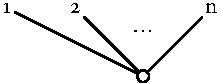
\includegraphics{figures/t_pq-all}
    \caption[\PQ-tree that represents all permutations]{A \PQ-tree that represents all permutations of $\range{n}$.}
    \label{figure:pq-all}
\end{figure}

A general~\PQ-tree does not really help
since the \PQ-tree in \myref{figure:pq-all} (a single \PT-node) represents all permutations of $\range{n}$,
\ie the problem does not get easier.

Thus, we have to narrow down the possible permutations even more. In this section we only consider
\Q-trees and show that \probQTree, which is \probBook restricted to~\Q-trees,
can be solved in quadratic time. In order to do this, we provide a reduction of the problem to~\probTwoSat, the problem of checking a 2-CNF formula for satisfiability. 
The \probTwoSat problem is solvable in linear time as first shown by Krom~\cite{Krom67}.

\newProb{\probQTree}{A \probBook instance $I$ with vertices $V$ and a \Q-tree~$T$ with leaves~$V$.}{Is there a total order $<\,\in \pi(T)$ solving $I$?}
\newProb{\probPTree}{A \probBook instance $I$ with vertices $V$ and a \PT-tree~$T$ with leaves~$V$.}{Is there a total order $<\,\in \pi(T)$ solving $I$?}
\newProb{\probTwoSat}{A 2-\CNF Boolean formula \bool{f}.}{Is~\bool{f} satisfiable?}

\Q-Trees are exactly the wrong type of trees
compared to the reformulation of the \SEFECON problem by Angelini et.\,al.~\cite{angelini11} since \Q-nodes vastly restrict the possible
permutations and are significantly easier to handle than \PT~nodes. This
section, therefore, only solves \SEFECON if the \PT-tree of the equivalent \probPTree instance is also a \Q-tree, \ie if the \PT-tree is a binary tree.

We first investigate what possible configurations of the leaves the book constraints 
lead to when we take the \Q-tree~$T$ into account. Then we show how these configurations
can be expressed with a 2-\CNF formula.

\paragraph{Possible configurations resulting from a book constraint}

\begin{figure}[\placement]\centering
    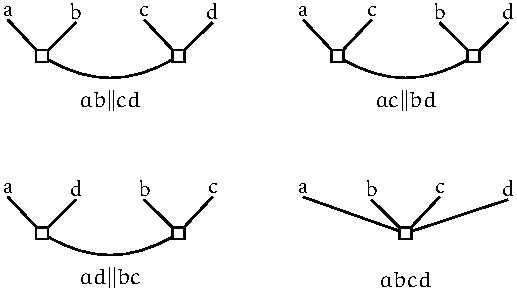
\includegraphics{figures/t_topo1}
    \caption[Topologies of four leaves]{The possible topologies of four leaves $a, b, c, d$ in a tree.}
    \label{figure:topo1}
\end{figure}


We first show that the book embedding restrictions for two edges $\{a, b\}$ and $\{c, d\}$
can be translated directly to restrictions on the $Q$-tree.
Before we start with this translation, however, we list some conventions. The \Q-tree is called $T$ and has leaves~$V$. Furthermore, let $t(M)$ be the smallest subtree of~$T$ containing~$M$ and let~$r(M)$ be its root for any~$M \subseteq V$.
Also remember that we assumed  in \myref{section:total-ordering} that any two edges we consider the book constraint for are independent.

%Consider the tree~$t(M)$ for~$M := \{a, b, c, d\}$.

We want to distinguish cases based on which two leaves in~$M := \{a, b, c, d\}$ can be separated from the others. These possible \emph{topologies of $M$ in~$T$} are depicted in \myref{figure:topo1}.
For example, we have~$ab||cd$ if there is an edge~$e \in E(T)$ such that $a$ and~$b$ are
in one component of~$T \setminus e$ while $c$ and~$d$ are in the other component, \ie
$a$ and~$b$ can be separated from $c$ and~$d$.
The topologies for $ac||bd$ and~$ad||bc$ are defined analogously. If no two vertices in~$M$ can be separated from the other
two (all pairs of vertices in~$M$ have the same lowest common ancestor) we say that the topology~$abcd$ occurs. 

%Thus, $t(M)$ has one of the trees in \myref{figure:topo1} as a
%topological minor, \ie the leaves $a$, $b$, $c$ and $d$ can appear
%in only a small number topological configurations. (Note that we do not take into consideration that the tree is rooted and ordered.) We call these configurations ``topologies'' below.

Depending on which of the topologies occurs, we can map the constraint from \myref{lemma:constraints} to a Boolean formula on the order~$<$ of the vertices~$V$.

\paragraph{Case 1: ab||cd}

Since $\{a, b\}$ and $\{c, d\}$ are in disjoint subtrees and the vertices of
a subtree are consecutive in every permutation $\pi(T)$, all tree orders
fulfil the book constraint. Thus, the constraint is mapped to the Boolean expression \bool{true}.

\paragraph{Case 2: ac||bd}

\begin{figure}\centering
    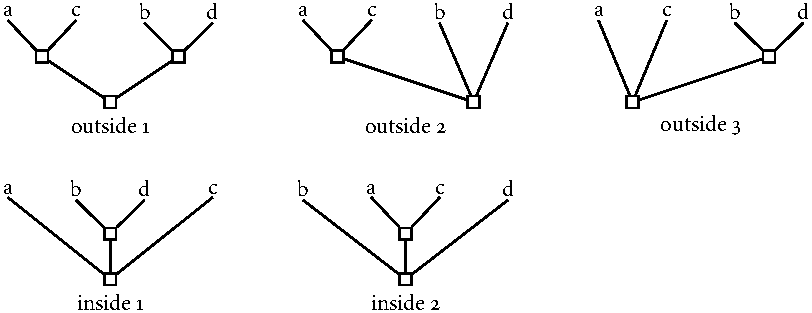
\includegraphics[scale=.9]{figures/t_order_ab_cd}
    \caption[Trees for $ac||bd$]{The possible trees corresponding to $ac||bd$.}
    \label{figure:order_ab_cd}
\end{figure}
\begin{figure}\centering
    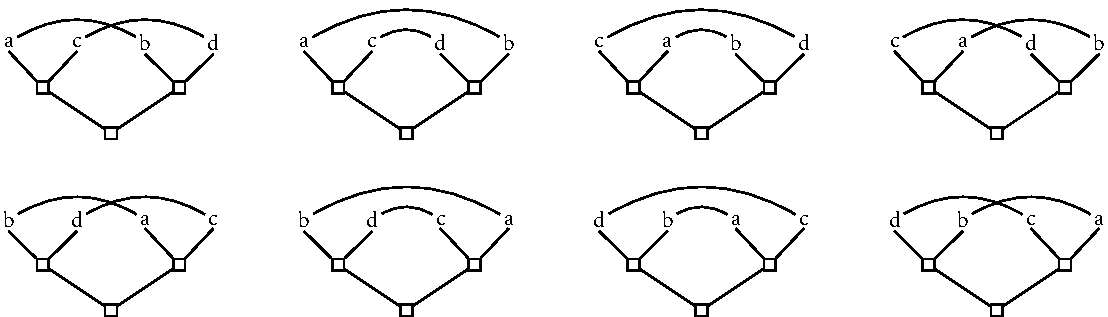
\includegraphics[width=\textwidth]{figures/t_topo_ac_bd}
    \caption[Outside 1 tree orders]{The tree orders for the case outside 1.}
    \label{figure:topo_ac_bd}
\end{figure}
\begin{figure}\centering
    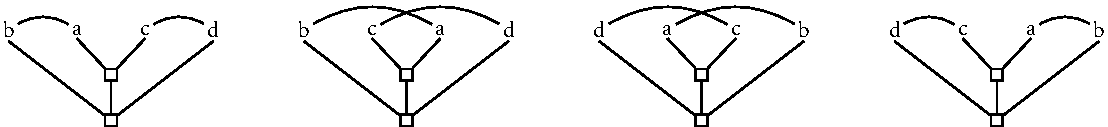
\includegraphics[width=\textwidth]{figures/t_topo_b_ac_d}
    \caption[Inside 1 tree orders]{The tree orders for the case inside 1.}
    \label{figure:topo_b_ac_d}
\end{figure}

In this case we search through the possible trees to determine the resulting
\probTwoSat formula. To do this systematically, we have to take into account that~$T$ is ordered and rooted and determine what the tree can look like. 

Thus, we further split this case into sub-cases based on whether the vertices $a$ and~$c$ are between $b$ and~$d$ (inside), $b$ and~$d$ are between $a$ and~$c$ (inside) or no two vertices in~$M$ are between the vertices they are separated from (outside). Note that $a$ and~$c$ are between $b$ and~$d$
for all orders in~$\pi(T)$ if they are between $b$ and~$d$ for one order in~$\pi(T)$ since~$T$
is a \Q-tree.

In the outside case, the
possible permutations also depend on how the roots of the subtrees $t(a, c)$ and $t(b, d)$ are related,
\ie whether one appears as a child of the other. The possible tree structures are depicted
in \myref{figure:order_ab_cd}.  
%We especially need not fix any portion of the order.

For each tree, we can exhaustively search through the orders of the leaves~$M$ the tree permits. For the 
case outside~1 these orders are portrayed in \myref{figure:topo_ac_bd}. We observe that the
valid orders are exactly the orders with $a < c \Leftrightarrow d < b$. The other two outside
cases can be handled similarly. Both of them again yield $a < c \Leftrightarrow d < b$.

For the inside cases we do the same. The possible orders of the case inside~1 are depicted in \myref{figure:topo_b_ac_d}. We can infer the
inverse $a < c \Leftrightarrow b < d$ for both inside cases. 

\paragraph{Case 3: ad||bc}

As in case~2, we either get $a < d \Leftrightarrow b < c$ or
$a < d \Leftrightarrow c < b$.

\paragraph{Case 4: abcd}

Let~$r$ be the common root $r(a, b, c, d)$ of $M := \{a, b, c, d\}$. The tree~$T$
represents two permutations of $M$ since the children of the \Q-node~$r$ can
only be reversed. If the book constraint is valid in a permutation of~$M$, it is also valid in the
mirror image of the permutation. Therefore, the book constraint may be valid in none or both of the two possible permutations. That is, we get either \bool{true} or
\bool{false} as constraint.

\paragraph{Mapping \probBook to \probTwoSat}

We now show how the resulting Boolean expressions can be mapped to \probTwoSat formulae.
To do so we fix a reference orientation of the inner nodes of~$T$.
For each $\pi \in \pi(T)$ and every inner node $v$ in $T$, we can say whether
we got $\pi$ as a permutation in~$\pi(T)$ by giving~$v$ the reference orientation or not.
Introduce a Boolean variable $o_v$ that stands for~$v$ being in reference orientation.

By the construction above, a book constraint for two edges yields one of the following Boolean expressions dependent on the structure of~$T$.

\begin{enumerate}
  \item A trivial expression \bool{true} or \bool{false}. (from cases~1 and~4)
  \item A fixed order of two leaves $v$ and~$w$ which is the same
  as fixing the order of their root~$r := r(v, w)$. Thus, we get
  $o_r$ or $\lnot o_r$. (from case~4)
  \item A connection between the orders of the leaves $a$, $b$ and $c$, $d$
  that are located in disjoint subtrees. This is the same as tying the
  orders of the roots $r := r(a, b)$ and $s := r(c, d)$ together.
  We get either $o_r \Leftrightarrow o_s \equiv (\lnot o_r \lor o_s) \land (\lnot o_s \lor o_r)$
  or $o_r \Leftrightarrow \lnot o_s \equiv (\lnot o_r \lor \lnot o_s) \land (o_s \lor o_r)$. (from cases~2 and~3)
\end{enumerate}

Thus, we can reduce \probQTree to determining whether a set of 2-\CNF expressions
is consistent with a \Q-tree structure. But since the inner nodes of a \Q-tree can be flipped completely independently of each other, the consistency with the \Q-tree structure does not
impose any extra restrictions. That is, \probQTree can be mapped to checking
a \probTwoSat formula for consistency (satisfiability).


%\newProb{\probQTreeSat}{A \Q-tree $T$ and a 2-\CNF expression $m$ on $\{o_v\colon \text{$v$ 
%is inner node of $T$}\}$ with $o_v$~signifying that the node~$v$ is ordered as in the initial tree.}{Is there a permutation in~$\pi(T)$ where~$m$ is satisfied?}

We now see how the reduction from \probQTree to \probTwoSat above can be 
implemented in qua\-dratic time.

\begin{lemma}
\label{lemma:q-tree-redux}
\probQTree can be reduced to \probTwoSat in quadratic time.
%A $\probQTree$~instance  can be reduced
%to a $\probTwoSat$ instance in $\OO\bigl(|T| + |E_1|^2 + \dotsb + |E_k|^2\bigr)$~time.
\end{lemma}
\begin{myproof}
Let $\bigl((V, E_1),\dotsc, (V, E_k), T\bigr)$ be an instance of $\probQTree$.
We can map the book constraints for each pair $e_1, e_2 \in E_i$ of edges for all
$i \in \range{k}$ to a 2-\CNF formula with the construction above.

Let's investigate how this can be done efficiently. Our goal is
to map each book constraint resulting from a pair of edges to a 2-\CNF formula in constant
time after a linear time precomputation. 

We assume $V = \range{n}$ and that each inner node of the tree~$T$ 
contains a pointer to its parent and an (ordered) list of its children.
Furthermore, let~$r$ be the root of~$T$.

%\begin{Ualgorithm}[\placement]
%\caption{Class for rooted, ordered trees}\label{alg:tree}
%\DontPrintSemicolon
%
%\SetKwFor{Class}{class}{}
%
%\SetKwFunction{Tree}{Tree}
%\SetKwFunction{PTree}{Pointer to Tree}
%\SetKwFunction{VTree}{Vector of pointers to Tree}
%\SetKwFunction{MyInt}{Integer}
%
%\Class{\Tree}{parent: \PTree\;children: \VTree}
%\end{Ualgorithm}

To determine the topology of a quadruple of leaves, we need to know
the lowest common ancestor of certain pairs of nodes and their initial order.

The first problem has been studied extensively. Harel and Tarjan~\cite{Harel84} showed
the surprising result that lowest common ancestor queries can be answered in constant
time after a linear time precomputation, although their algorithm was too complicated to be implemented
effectively. Farach and Colton~\cite{Farach00} presented a far simpler variant of this
algorithm that is used in practice. We assume in the following that the precomputation has 
been done and that \algoFont{LCA($x$, $y$)} gives the lowest common ancestor of~$x$ and~$y$ in~$\OO(1)$ time.

For the second problem, we can precompute the index array~\algoFont{idx} of~$V$ that maps each
leaf~$V$ to its index in the reference orientation of~$T$. This can be accomplished in linear time by a simple depth-first search. 

%At each step,
%we know the index the leaves in the current subtree start with. We recurse on the children
%of the current node in order and update the starting index accordingly. When we arrive at a
%leaf, we know that its index is the current starting index, which is given as a parameter. The initial
%call is~\algoFont{ComputeIndex$(r, 1)$}.
%
%\begin{Ualgorithm}[\placement]
%\caption[Computing the index array]{Computing the index array: \algoFont{ComputeIndex}}\label{alg:index}
%
%\SetKwFunction{Tree}{Tree}
%\SetKwFunction{ComputeIndex}{ComputeIndex}
%\SetKwFunction{size}{size}
%\SetKwFunction{content}{idx}
%\SetKwFunction{children}{children}
%
%\SetKwData{T}{T}
%\SetKwData{firstIdx}{s}
%\SetKwData{lastIdx}{e}
%\SetKwData{idx}{idx}
%\SetKwData{mycnt}{i}
%
%\KwIn{Tree $T$, starting index $s$}
%\KwOut{Ending index $e$}
%
%\BlankLine
%\tcp{Is $T$ leaf?}
%\If{$\T.\children.\size = 0$}{
%$\lastIdx \leftarrow \firstIdx$ \;
%$\idx[\T.\content] \leftarrow \firstIdx$
%}
%\Else {
%	\tcp{Recurse and update indexes}
%	\For{$\mycnt \leftarrow 1$ to $\T.\children.\size$}{
%		$\firstIdx \leftarrow \ComputeIndex(\T[\mycnt], \firstIdx) + 1$
%	}
%}
%\end{Ualgorithm}

Before we begin with the actual translation, we need another helper function \algoFont{Leaf-Order($a$,$b$)} that translates a statement
of the form~$a < b$ for leaves $a, b \in V$ into a literal on the variable~$o_r$ 
where $r = \algoFont{LCA}(a, b)$. If $\algoFont{idx[a]} < \algoFont{idx[b]}$, then~$r$ has reference orientation and the result is~$o_r$. Otherwise, the result is~$\lnot o_r$. This decision can obviously
can be made in $\OO(1)$~time.

%\begin{Ualgorithm}[\placement]
%\caption[Literal for leaf order]{A literal for a given leaf order: $\algoFont{Leaf-Order}$}\label{alg:lca}
%
%\KwIn{Leaves $a, b \in V$}
%\KwOut{A Boolean formula representing $a < b$}
%
%\SetKwFunction{LCA}{LCA}
%
%\SetKwData{firstPar}{a}
%\SetKwData{secondPar}{b}
%\SetKwData{idx}{idx}
%
%\BlankLine
%$r \leftarrow \LCA(\firstPar, \secondPar)$ \;
%\If{$\idx[\firstPar] < \idx[\secondPar]$}{
%	\KwRet $o_r$
%}
%\Else{
%	\KwRet $\lnot o_r$
%}
%\end{Ualgorithm}

We now have everything we need to translate book constraints into
Boolean formulae. The direct formalisation of the construction
above is given in \myref{alg:translate}. It returns
a Boolean formula for a pair of edges $\{a, b\}$ and~$\{c, d\}$
in~$\OO(1)$. Note that we can test whether the order~\algoFont{idx} fulfils
the book constraint in line~9 in~$\OO(1)$ time since only the relative
order of $a$, $b$, $c$ and $d$ is relevant.

In the algorithm, the Boolean formulae are not given in conjunctive normal
form for the sake of clarity. If we want \CNF~formulae, we can statically replace
the Boolean formulae in \myref{alg:translate} by their \CNF~equivalents.


\SetAlFnt{\footnotesize\sf}
\begin{Ualgorithm}[\placement]
\caption[Translating the book constraint in $\OO(1)$]{Translating the book constraint in $\OO(1)$ }\label{alg:translate}

\SetKwFunction{LCA}{LCA}
\SetKwFunction{LeafOrder}{Leaf-Order}

\SetKwData{pa}{a}
\SetKwData{pb}{b}
\SetKwData{pc}{c}
\SetKwData{pd}{d}
\SetKwData{idx}{idx}

\KwIn{Two edges $\{\pa, \pb\}$ and $\{\pc, \pd\}$}
\KwOut{A Boolean formula representing the book constraint for the two edges}

\BlankLine

\tcp{Independent edges?}
\If{$|\{\pa, \pb, \pc, \pd\}| = 4$}{
	$r_1 \leftarrow \LCA(\pa, \pb)$ \;
    $r_2 \leftarrow \LCA(\pa, \pc)$ \;
	$r_3 \leftarrow \LCA(\pa, \pd)$ \;
	$r_4 \leftarrow \LCA(\pb, \pc)$ \;
	$r_5 \leftarrow \LCA(\pb, \pd)$ \;
	$r_6 \leftarrow \LCA(\pc, \pd)$ \;
	\If{all~$r_i$ are the same for~$i \in \range{6}$}{
		\tcp{$abcd$}
%		$x \leftarrow \text{leaf with smallest \idx among \pa, \pb, \pc and \pd}$ \;
%		$y \leftarrow \text{leaf with largest \idx among \pa, \pb, \pc and \pd}$ \;
		\If{Order \idx fulfils book constraint}{
			\KwRet $true$
		}
		\Else{
			\KwRet $false$
		}
	} \ElseIf{$\LCA(r_2, r_5)$ is not equal to $r_2$ or $r_5$}{
		\tcp{$ac||bd$}
		\If{$\idx[\pa]$ between $\idx[\pb]$ and $\idx[\pd]$}{
			\KwRet $\LeafOrder(\pa, \pc) \Leftrightarrow \LeafOrder(\pb, \pd)$
		}
		\Else {
			\KwRet $\LeafOrder(\pa, \pc) \Leftrightarrow \LeafOrder(\pd, \pb)$
		}
	} \ElseIf{$\LCA(r_3, r_4)$ is not equal to $r_3$ or $r_4$}{
	    \tcp{$ad||bc$}
	    \If{$\idx[\pa]$ between $\idx[\pb]$ and $\idx[\pc]$}{
			\KwRet $\LeafOrder(\pa, \pd) \Leftrightarrow \LeafOrder(\pb, \pc)$
		}
		\Else {
			\KwRet $\LeafOrder(\pa, \pd) \Leftrightarrow \LeafOrder(\pc, \pb)$
		}
	} \Else {
	    \tcp{$ab||cd$}
		\KwRet $true$
	}
}
\Else{
	\KwRet $true$
}
\end{Ualgorithm}

All in all, we need~$\OO\bigl(|T|\bigr)$ time for the precomputation and
$\OO(1)$~time for each of the~$\OO\bigl(|E_1|^2+\dotsb+|E_k|^2\bigr)$ book constraints.
Thus, the reduction to \probQTreeSat takes $\OO\bigl(|T| + |E_1|^2 + \dotsb + |E_k|^2\bigr)$~time.\qedhere
%We need to determine the topological structure of each of the
%$|E_1|^2 + \cdots + |E_n|^2$ edge pairs $e_1$ and $e_2$. This
%can be done in~$\OO(|T|)$ by following a path from a vertex of $e_1$ to the root
%if we have a bit-field of length $\OO(|V|)$ for each inner node $v$~of~$T$ from which we
%can determine, whether a leaf is contained in the subtree rooted at~$v$. The bit-field
%can be recursively precomputed in time $\OO(|T|^2|V|)$.

%Thus, the reduction to \probQTreeSat takes $\OO(|T|\cdot(|E_1|^2 + \cdots + |E_n|^2 + |V||T|))$~time
\end{myproof}

%The problem~\probQTreeSat is clearly efficiently solvable.

%\begin{lemma}
%An instance~$(T, m)$ of \probQTreeSat can be solved in $\OO\bigl(|m|\bigr)$.
%\end{lemma}
%\begin{myproof}
%The inner nodes of~$T$ can be flipped completely independently of each other,
%\ie there are no constraints on the~$o_v$ except the ones given in~$m$.
%Since~$m$ is a 2-\CNF expression, checking it for consistency (satisfiability)
%can be done in $\OO\bigl(|m|\bigr)$ as first shown by Krom~\cite{Krom67}.
%\end{myproof}

Since \probTwoSat is solvable in linear time, we conclude that \probQTree can be solved in quadratic time.

\begin{theorem}
\label{theorem:q-tree-book}
\probQTree can be solved in quadratic time.
\end{theorem}
\begin{myproof}
Let $\bigl((V, E_1),\dotsc, (V, E_k), T\bigr)$ be an instance of $\probQTree$.
We saw that the reduction to \probTwoSat takes $\OO\bigl(|T| + |E_1|^2 + \dotsb + |E_k|^2\bigr)$ time
in \myref{lemma:q-tree-redux}. For each pair of edges $e_1, e_2 \in E_i$ where $i \in \range{n}$ we get a 2-\CNF expression of length $\OO(1)$. Since \probTwoSat is solvable in linear
time as first shown by Krom~\cite{Krom67}, we, therefore, need $\OO\bigl(|E_1|^2 + \dotsb + |E_n|^2\bigr)$~time to solve the resulting \probTwoSat problem.
Altogether, we need $\OO\bigl(|T| + |E_1|^2 + \dotsb + |E_k|^2\bigr)$ time.
\end{myproof}

We have assumed $|E_i| \le 2|V|-3$ for all~$i \in \range{k}$ at the
start of \myref{ch:preliminaries} since the pages
have to be outerplanar to be embeddable. Furthermore, the \Q-tree 
has fewer inner nodes than its number of leaves~$|V|$ since each inner node
has at least two children.
That is, we can rewrite the time as
$\OO\bigl(|T| + |E_1|^2 + \dotsb + |E_k|^2\bigr) = \OO\bigl(|V| + k(2|V|-3)^2\bigr) = \OO\bigl(k|V|^2\bigr)$.

\paragraph{Outlook}

So book embedding is solvable in quadratic time if we constrain the vertex order by a \Q-tree. But what if we have a \PT-tree as in the
reformulation of \SEFECON? We have already seen in \myref{figure:pq-all} that this
restriction cannot make the problem simpler than the general book embedding problem. Furthermore, we cannot directly generalise our construction since the answer to ``What permutation of the children of a \PT-node occurs?'' cannot simply be modelled by a Boolean variable.
%for example, the sub-argument for $ac||bd$ depends on us being able to distinguish between the inside
%and outside cases. If the common root $r := r(a, b, c, d)$ were a \PT-node, the tree would
%allow permutations with $ac$ between~$bd$ and permutations where this is not the case, \ie there are %valid
%orders with $a < c \land b < d$ and ones with $a < c \land d > b$. This means that we cannot simply
%model the book constraint by looking at how~$r$ is flipped.
That is, \probPTree remains an
interesting open problem.